\documentclass{article}
\usepackage{times}
\usepackage[nohead,bottom=3cm,top=2cm,a4paper]{geometry}
\usepackage{enumerate}
\usepackage{nicefrac}
\usepackage{xcolor}
\usepackage{graphicx}
\usepackage[nswissgerman]{babel}
\usepackage{listings}
\usepackage{caption}
\usepackage{subcaption}
\usepackage{lipsum}


% for matlab source-code
\newcommand{\matlab}[1]{%
\begin{small}
\lstinputlisting[caption={\texttt{#1}},basicstyle={\ttfamily},commentstyle={\color{black!50!green}\itshape},frame=tb,keywordstyle={\color{black!60!blue}\bfseries},stringstyle=\color{black!60!orange},language=Matlab,breaklines=true,numbers=left,numberstyle={\color{black!50!white}}]{#1}%
\end{small}
}



\title{Resultate aus dem Projekt zu ``Einf\"uhrung in die Numerik'', FS24}
\author{Ephraim Siegfried}

\begin{document}
\maketitle


\section*{Aufgabe 1: Simulation eines Schwarms}
\begin{figure}[h]
	\begin{subfigure}{0.5\textwidth}
		\centering
		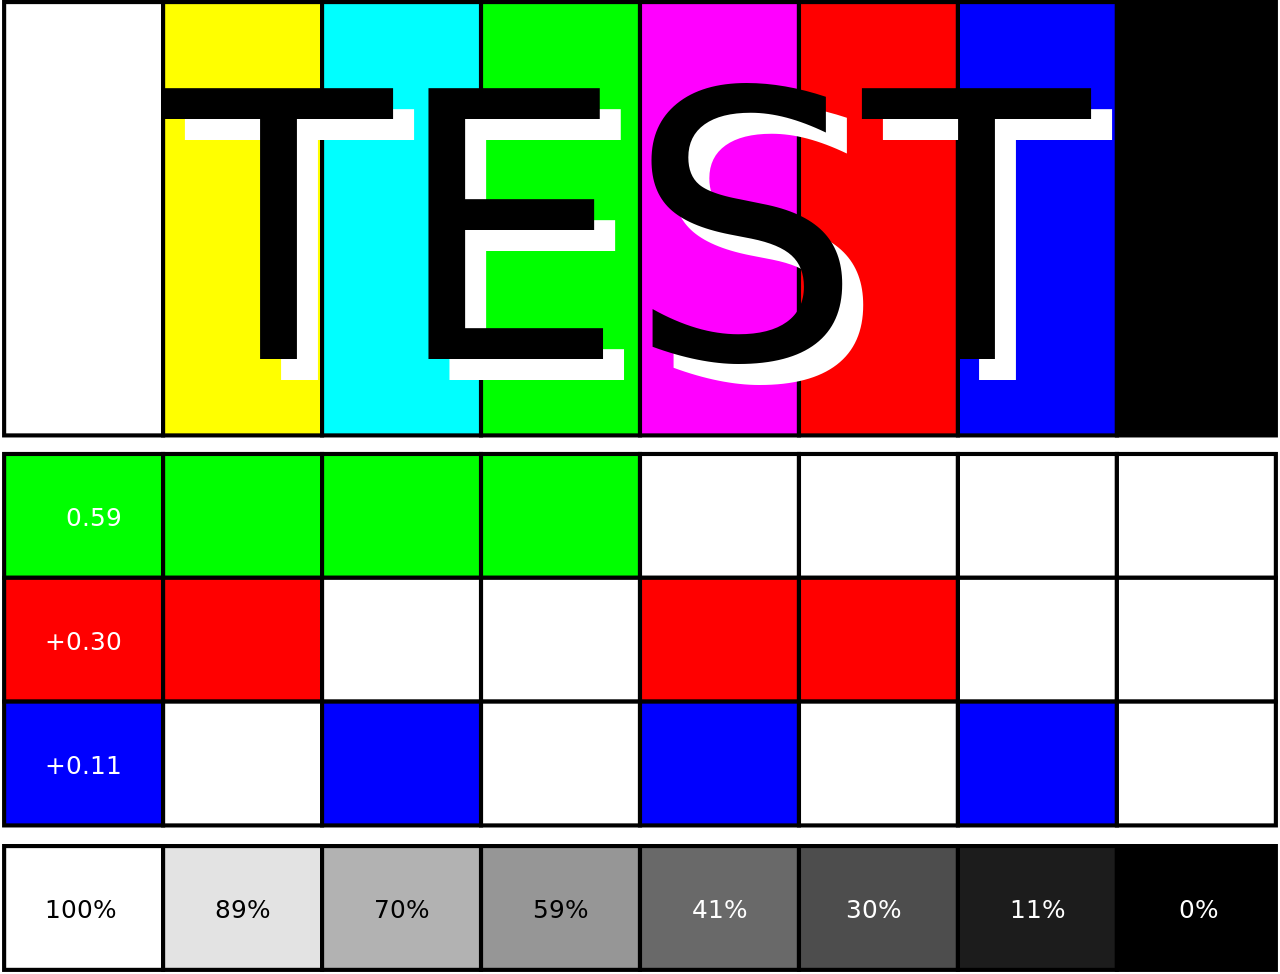
\includegraphics[width=\textwidth]{figures/placeholder.png}
	\end{subfigure}
	\begin{subfigure}{0.5\textwidth}
		\centering
		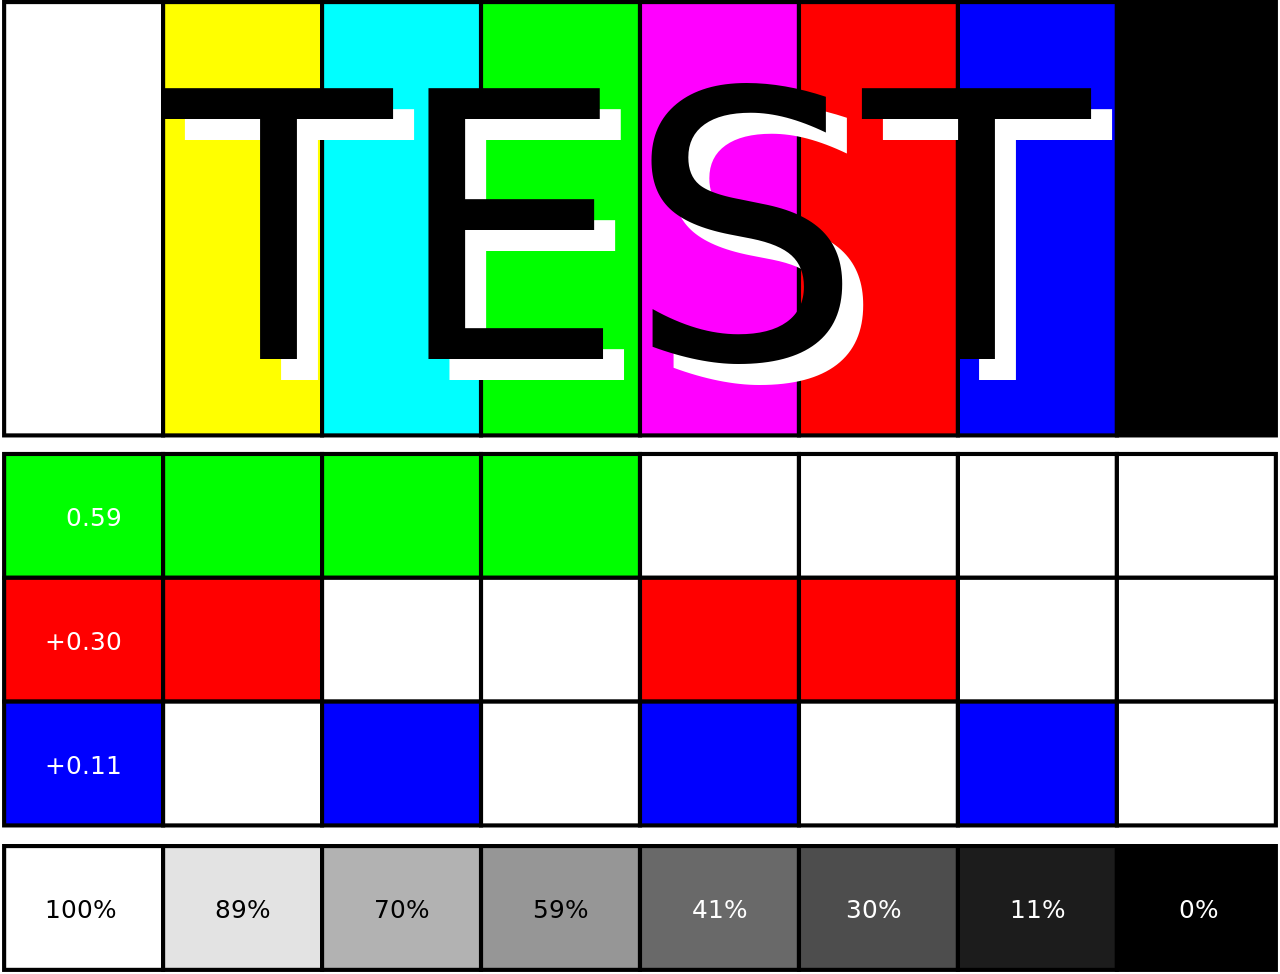
\includegraphics[width=\textwidth]{figures/placeholder.png}
	\end{subfigure}
	\caption{
		\lipsum[66]
	}
\end{figure}

\lipsum[1]
% ToDo: Loesche den Befehl lipsum und fuege hier deine Antworten auf die Fragen ein.

\section*{Aufgabe 2: Einfacher Wurf}
\lipsum[2]
% ToDo: Loesche den Befehl lipsum und fuege hier deine Antworten auf die Fragen ein.

\section*{Aufgabe 3: Ein springender Ball}
\lipsum[3]
% ToDo: Loesche den Befehl lipsum und fuege hier deine Antworten auf die Fragen ein.

\section*{Aufgabe 4: Luftwiderstand}
\lipsum[4]
% ToDo: Loesche den Befehl lipsum und fuege hier deine Antworten auf die Fragen ein.

\section*{Aufgabe 5: K\"orbe werfen}
\begin{table}[h!]
	\centering
	\begin{tabular}{l || l | l | l }
		\(\Delta t^{(1)}\) & i  & \({\bf x}^{(i)}-x^{(1)}\) & \({\bf v}^{(i)}\) \\
		\hline
		0.1                & 10 & 2m                        & 4m/s              \\
		0.01               & 20 & 3m                        & 3m/s              \\
		0.001              & 30 & 4m                        & 2m/s
	\end{tabular}
	\caption{Anzahl an Iterationen, Wurfdistanz, Endgeschwindigkeit und Schrittweite f\"ur das explizite Euler-Verfahren zum Zeitpunkt an dem der Ball zum ersten Mal den Boden ber\"uhrt. Beim Abwurf: Entfernung \ldots m, H\"ohe \ldots m, Winkel \ldots$^\circ$ und Geschwindigkeit \ldots m$/$s. }
	\label{tab:expEul}
\end{table}
\begin{table}[h!]
	\centering
	\begin{tabular}{l || l | l | l }
		\(\Delta t^{(1)}\) & i  & \({\bf x}^{(i)}-x^{(1)}\) & \({\bf v}^{(i)}\) \\
		\hline
		0.1                & 10 & 2m                        & 4m/s              \\
		0.01               & 20 & 3m                        & 3m/s              \\
		0.001              & 30 & 4m                        & 2m/s
	\end{tabular}
	\caption{Anzahl an Iterationen, Wurfdistanz, Endgeschwindigkeit und Schrittweite f\"ur das Heun-Verfahren zum Zeitpunkt an dem der Ball zum ersten Mal den Boden ber\"uhrt. Beim Abwurf: Entfernung \ldots m, H\"ohe \ldots m, Winkel \ldots$^\circ$ und Geschwindigkeit \ldots m$/$s. }
	\label{tab:Heun}
\end{table}
\begin{table}[h!]
	\centering
	\begin{tabular}{l || l | l | l }
		\(\Delta t^{(1)}\) & i  & \({\bf x}^{(i)}-x^{(1)}\) & \({\bf v}^{(i)}\) \\
		\hline
		0.1                & 10 & 3m                        & 3m/s              \\
		0.01               & 10 & 3m                        & 3m/s              \\
		0.001              & 10 & 3m                        & 3m/s
	\end{tabular}
	\caption{Anzahl an Iterationen, Wurfdistanz, Endgeschwindigkeit und Schrittweite f\"ur das RKF2(3)-Verfahren zum Zeitpunkt an dem der Ball zum ersten Mal den Boden ber\"uhrt. Beim Abwurf: Entfernung \ldots m, H\"ohe \ldots m, Winkel \ldots$^\circ$ und Geschwindigkeit \ldots m$/$s. }
	\label{tab:RKF2(3)}
\end{table}
\lipsum[5]
% ToDo: Loesche den Befehl lipsum und fuege hier deine Antworten auf die Fragen ein.

\begin{figure}[h]
	\centering
	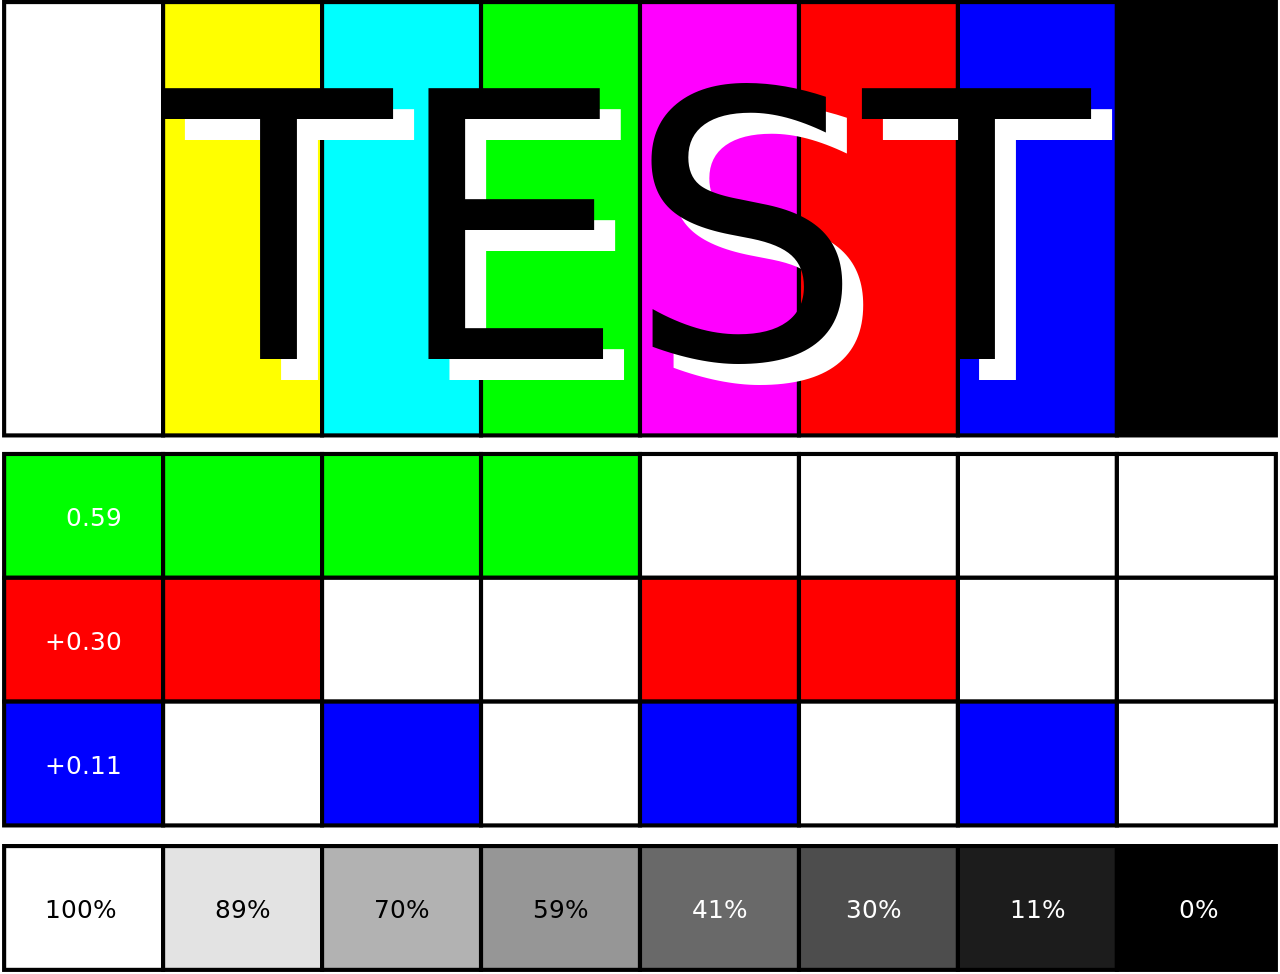
\includegraphics[width=\textwidth]{figures/placeholder.png}
	\caption{Basketballwurf einmal ohne Luftwiderstand (\textcolor{blue}{*}) und einmal mit (\textcolor{magenta}{o}).}
\end{figure}



\newpage
\section*{Quellcode}
\matlab{../src/sysDiffGlgen.m}
\matlab{../src/explEulSchwarm.m}
\matlab{../src/heunSchwarm.m}
% \matlab{../src/A1_1.m}
\end{document}
